\svnidlong
{$HeadURL$}
{$LastChangedDate$}
{$LastChangedRevision$}
{$LastChangedBy$}
\svnid{$Id: $}


%%%%%%%%%%%%%%%%%%%%%%%%%%%%%%%%%%%%%%%%%%%%
%\section*{EFT Validity and Truncation Summary}
%%%%%%%%%%%%%%%%%%%%%%%%%%%%%%%%%%%%%%%%%%%%

Most of this report has focused on simplified models.
In this Chapter, we wish to emphasize the applicability of
Effective Field Theories (EFTs) 
in the interpretation of DM searches at the LHC.
Given our current lack of knowledge about the nature of a DM particle and
its interactions, it appears mandatory to provide the necessary information
for a model independent interpretation of the collider bounds.
This approach should be complemented with
an interpretation within a choice of simplified models.
We note that, even though EFT benchmarks are only valid in given conditions,
the results provided by the current list of simplified models cannot always
characterize the breadth of SM-DM interactions.
In at least one case, composite WIMPs~\cite{Nussinov:1985xr,Kaplan:1991ah,Banks:2010eh}, 
the contact interaction framework is the correct one to
constrain new confinement scales. 

%Even when the application of EFT is not appropriate for the prediction of kinematics 
%or cross sections, it does predict specific final states and can motivate experimental searches.

Ideally, experimental constraints should be shown as bounds of allowed signal events in the kinematic regions considered for 
the search, as detailed in Appendix~\ref{app:Presentation_Of_Experimental_Results}. 
A problematic situation is the attempt to derive a limit on
nucleon-dark matter scattering cross sections from EFT results
based on collider data~\footnote{Comparisons between constraints from different experiments 
	meant to highlight their complementarity should be expressed as 
	a function of the model parameters rather than on derived observables;
	however this is a point that should be developed further after the conclusion of the work of this Forum.}. 
Experiments that directly probe the nucleon-dark matter scattering cross section 
are testing the regime of small momentum transfers, where the EFT approximation always holds.  
Collider experiments, though, are sensitive to large momentum transfers: this is a regime where careful 
treatment is necessary since the condition of applicability of the EFT may not hold.\footnote{
Furthermore, mapping EFT results from high to low momentum requires particular care for some of the operators, 
see Ref.~\cite{D'Eramo:2014aba} for a thorough discussion.}
Therefore, especially in the case when constraints from different experiments are compared, 
we suggest to assess the applicability of EFT benchmark models, rather than abandon them.
%As we have learned, EFTs do not truly represent a model-independent representation of the data for the current collider sensitivity.
%Until the various communities have agreed upon how to present this comparison, 
Therefore, whenever EFT models are used, collider experiments should always assess their applicability 
using one 
of the several prescriptions in the literature~\cite{Busoni:2013lha,Busoni:2014sya,Busoni:2014haa,Aad:2015zva,Racco:2015dxa}, 
especially when constraints from other experiments are compared.

We first illustrate the complications
that can arise with EFTs at colliders by considering an effective interaction
$$ {\cal L}_\textrm{int} = {(\bar q\gamma_\mu q)(\bar\chiDM\gamma^\mu\chiDM) \over \Mstar^2}
= (\bar q\gamma_\mu q)(\bar\chiDM\gamma^\mu\chiDM) {g\over \Lambda^2}$$
that couples quarks and DM $\chi$ fields.\footnote{The \textit{exact} operator chosen is not important.}   The strength of this interaction is
parametrized by $\displaystyle {1\over \Mstar^2} = {g\over \Lambda^2}$.
A monojet signature can be generated from this operator
by applying perturbation theory in the QCD coupling.
An experimental search will place a limit on \Mstar.   
For a fixed \Mstar, a small value of $g$ will correspond
to a small value of $\Lambda$.   The EFT approximation breaks down
if $Q>\Lambda$, where $Q$ is a typical hard scale of the process.
%One possible example is $\Qtr^2=[p(\bar\chiDM\chiDM)]^2$, i.e.
%the momentum flow through
%the \schannel.% asked by Davide to remove this as its not correct.
The limit on small $g$ can only be reliable if the
kinematic region $Q>\Lambda$ is removed from the event generation.
However, if a fraction of events is removed from the prediction,
the corresponding value of $g$ must increase to match the experimental
limit on \Mstar.
On the other hand, if, for the same value of \Mstar, a large $\Lambda$
is assumed so that the full set of events fulfill the EFT validity condition,
a large value of
$g$ is required, raising the question if perturbation theory
is even applicable.     

In the first part of this Chapter, we summarize two methods that
have been advocated to truncate events that 
do not fulfill the condition necessary for the use of an EFT.
% and improve the reliability of the approximation by delivering conservative results. 
These methods are described in detail in Refs.~\cite{Busoni:2013lha,Busoni:2014sya,Busoni:2014haa,Aad:2015zva,Racco:2015dxa,Berlin:2014cfa}. 
We then propose a recommendation for the presentation of EFT results for early Run-2 LHC searches.

\section{Procedures for the truncation of EFT benchmark models}

%%%%%%%%%%%%%%%%%%%%%%%%%%%%%%%%%%%%%%%%%%%%
%\section{\texorpdfstring{Outline of the procedure described in Refs.~\cite{Busoni:2014sya,Aad:2015zva}}{Outline of the procedure described in Refs.}}
%CD: qualify the procedure
\subsection{EFT truncation using the momentum transfer and information on UV completion}

\label{sec:TruncationWithQTr}
%%%%%%%%%%%%%%%%%%%%%%%%%%%%%%%%%%%%%%%%%%%%

%The approach described in Refs.~\cite{Busoni:2014sya,Aad:2015zva} 
%predates the implementation of simplified models, 
%and can be viewed as a stop-gap measure until the simplified models could be fully simulated.
%CD: I am not sure of this sentence, because the simplified models were there but we were just not using them. 
In the approach described in Ref.~\cite{Busoni:2014sya},
the EFT prediction is modified to incorporate the effect of a
propagator for a relatively light mediator.
For a tree-level interaction between DM and
the SM via some mediator with mass \mMed, 
the EFT approximation corresponds to expanding the propagator
for the mediator
in powers of $\Qtr^2/\mMed^2$, truncating at lowest order, and combining the remaining parameters into a single parameter \Mstar 
(connected to the scale of the interaction $\Lambda$ in the literature).
For an example scenario with a \Zprime-type mediator (leading to some combination of operators D5 to D8 in the notation of~\cite{Goodman:2010ku} for the EFT limit),
this corresponds to setting
\be
\frac{\gDM \gq}{Q_{\rm tr}^2-\mMed^2}=-\frac{\gDM \gq}{\mMed^2}\left(1+\frac{Q^2_{\rm tr}}{\mMed^2}+ \mathcal{O} \left(\frac{Q^4_{\rm tr}}{\mMed^4}\right)\right) \simeq -\frac{1}{{\Mstar^2}},
\ee
%
where $\Qtr$ is the momentum carried by the mediator, and $\gDM$,
$\gq$ are the DM-mediator and quark-mediator couplings
respectively.\footnote{Here, we ignore potential complications from
the mediator width when the couplings are large.}
%Similar expressions exist for other operators.
A minimal condition that must be satisfied for this approximation to be valid is that $\Qtr^2 < \mMed^2 = \gDM \gq {\Mstar^2}$.
This requirement avoids the regions:
$\Qtr^2 \sim \mMed^2$, in which case the EFT misses a resonant enhancement, and it is conservative to ignore this enhancement;
and $\Qtr^2 \gg \mMed^2$, in which case the signal cross section
should fall according to a power of $\Qtr^{-1}$ instead of $\mMed^{-1}$.   The latter is the problematic kinematic region.

The condition $\Qtr^2 < \mMed^2 = \gDM \gq \Mstar^2$ was applied
to restrict the
kinematics of the signal and remove events for which the high-mediator-mass approximation made in the EFT would not be reliable.
This leads to a smaller effective cross-section, after imposing the event selection of the analysis.  This truncated signal was then used
to derive a new, more conservative limit on
$\Mstar$ as a function of $(\mDM, \gDM \gq)$.
%TODO SM: I am uncomfortable with saying ``ensure the validity.'' CD: me too. However "improve the reliability of the validity" is cumbersome so I changed it.

For the example D5-like operator,
where the cross section $\sigma$ scales as $\Mstar^{-4}$,
there is a simple rule for converting a rescaled cross section into a rescaled constraint on ${\Mstar}$.
if the original limit is based on a simple cut-and-count procedure.
%CD: I would keep it
Defining $\sigma_{\rm EFT}^{\rm cut}$ as the cross section truncated such that all events pass the condition $\sqrt{\gDM \gq} \Mstar^{\rm rescaled} > \Qtr$, we have
\be
\Mstar^{\rm rescaled} = \left(\frac{\sigma_{\rm EFT}}{\sigma_{\rm EFT}^{\rm cut}(\Mstar^{\rm rescaled})}\right)^{1/4} \Mstar^{\rm original},
\ee
%
which can be solved for $\Mstar^{\rm rescaled}$ via either iteration or a scan.
%(note that $\Mstar^{\rm rescaled}$ appears on both the LHS and RHS of the equation).
Similar relations exist for a given UV completion of each operator. The details and application of this procedure to 
ATLAS results can be found in Ref.~\cite{Aad:2015zva} for a range of operators.
We reiterate: knowledge of the UV completion for a given
EFT operator was necessary for this procedure;
this introduces a model-dependence that was not present
in the non-truncated EFT results. 

%CD: Tim's reasoning is below. 
%You argued (well, reported on an argument) that the use of the EFT somehow is a barrier to collider searches being appreciated by colleagues who work on other detection strategies.  Of course, I do not know what the future will hold under any scenario, but I strongly believe that the rejection of the collider bounds is based entirely on politics by the direct detection community, who feels threatened that it weakens their designs to expand to lower mass.  Of course, so far they are getting funding to do that anyway, so they should not feel threatened, but they do not want the competition.
%
%My prediction is that by going from an EFT to a simplified model, the response from colleagues in other fields will be that the mapping is (self-evidently) model-dependent, and therefore they do not want to include it since it is at odds with their “direct” limits.  This objection is essentially false in the sense that even when they compare one experiment to each other, it is model-dependent, but it is true that the model is more manifestly important here.
%
%I think the better strategy is going to be to use the language of the models (rather than observables) as the comparison point.  This will be much less political, and it can turn into a limit from each experiment on the cut-off scale as a function of mass for the EFT, or masses and couplings in a given simplified model.  The complementarity of experiments will be manifest there, but no one will need to feel territorial about their own turf.
%
%I also object to framing the discussion of the EFT as a discussion of “validity”.  The EFT is valid only as a proxy for a given model, and to ask the question as just the EFT being valid or invalid at the LHC is a question without any meaningful well-defined answer.  To ask how well it does requires one to know the model that describes higher energies, and this is a case where we don’t have that information — which is the point!  I appreciate that what you are advocating to do in practice is the correct thing (and what I have also advocated for all along), but to frame it as a question of validity of the LHC results on EFTs is very misleading and contributes ammunition to those people such as the one I mentioned before who are very confident shouting about things they do not understand.
 
%Since this method uses the physical couplings and energy scale $\Qtr$, it gives the strongest possible constraints in the EFT limit while remaining robust by ensuring the validity of the EFT approximation.
%TODO: Too strong of a statement? CD: more like - this does not parse. Removed.

Currently, simplified models (including the full effect
of the mediator propagator) are available for comparison with
the data, and since knowledge of the simplified models is needed
for the truncation procedure,
there is no reason to apply this prescription.   Instead, the
simplified model limit for large \Mstar can be presented for
interpretation in terms of EFT operators.


%%%%%%%%%%%%%%%%%%%%%%%%%%%%%%%%%%%%%%%%%%%%
\subsection{EFT truncation using the center of mass energy}
\label{sec:TruncationWithSHat}
%%%%%%%%%%%%%%%%%%%%%%%%%%%%%%%%%%%%%%%%%%%%

The procedure presented in the previous section was predicated on
some knowledge of the simplified model.  This led to the identification
of the mass of the DM pair as the relevant kinematic quantity to use
in a truncation procedure.
In general, if no assumption is made about the underlying dynamics,
it is more conservative to place a limit on the total center
of mass energy $E_\text{cm}$ of the DM production process.
Furthermore, the direct connection between the mass scale of
the EFT validity, \Mcut, and the
mass scale that normalizes the EFT operator, \Mstar, is unknown.
For such cases,~Refs.\cite{Racco:2015dxa,Berlin:2014cfa} proposed
a procedure to extract model independent and consistent bounds within the EFT
that can be applied to any effective Lagrangian describing the interactions between the DM and the SM.
This procedure provides conservative limits that can be directly reinterpreted in any completion of the EFT.
The condition ensuring that the EFT approximation is appropriate is:
\begin{equation}
\label{Ecm<Mcut}
E_\text{cm}<M_\text{cut}\,.
\end{equation}

%% For example, in the specific case of a tree level mediation with a single mediator, \Mcut can be interpreted as the mass of that mediator.

%% There are then at least three free parameters describing an EFT:~ 
%% the DM mass $m_\text{DM}$, the scale $\Mstar$ of the interaction, and the scale \Mcut.

%% We can use the same technique as above to restrict the signal to the events for which $E_\text{cm}<M_\text{cut}$,  using only these events to derive the exclusion limits on $\Mstar$ as a function of  $(m_\text{DM},M_{\rm cut})$. 
%
The relationship between \Mcut and \Mstar can be parameterized
by an \textit{effective coupling strength} \gstar, such that
$\Mcut=\gstar \, \Mstar\,.$
A scan over values of \gstar provides an indication of the
sensitivity of the prediction to the truncation procedure.
In the \Zprime-type model considered above, \gstar is equal to $\sqrt{\gDM\gq}$.
%
The resulting plots are shown in \cite{Racco:2015dxa} for a particular effective operator. 

The advantage of this procedure is that the obtained bounds can be directly and easily recast in any  completion of the EFT, by computing the parameters \Mstar, \Mcut in the full model as functions of the parameters of the complete theory. On the other hand, the resulting limits will be weaker than those obtained using \Qtr and a specific UV completion.

\subsection{Consideration for shape analyses}

If a search is not simply a counting experiment and exploits the shapes of kinematic distributions, any of the two conditions on the momentum transfer should be applied on the benchmarks using generator level information, by discarding events that are invalid, and the limit derived from
the truncated shape must be recalculated. This provides the necessary rescaling of the cross section while keeping the information on the change in the kinematic distributions due to the removal of the invalid events. 

\subsection{Sample results of EFT truncation procedures}

An example of the application of the two procedures to the limit on $M_*$ from Ref.~\cite{ATL-PHYS-PUB-2014-007} as a function of the product of the couplings is shown in Figure~\ref{Ecm<Mcut}. Only the region between the dashed and the solid line is excluded. It can be seen that the procedure from~\cite{Racco:2015dxa} outlined in Section~\ref{sec:TruncationWithSHat}, shown in blue, is more conservative than the procedure from Refs.~\cite{Busoni:2014sya,Aad:2015zva}, described in Section~\ref{sec:TruncationWithQTr}.

\begin{figure}
	\centering
	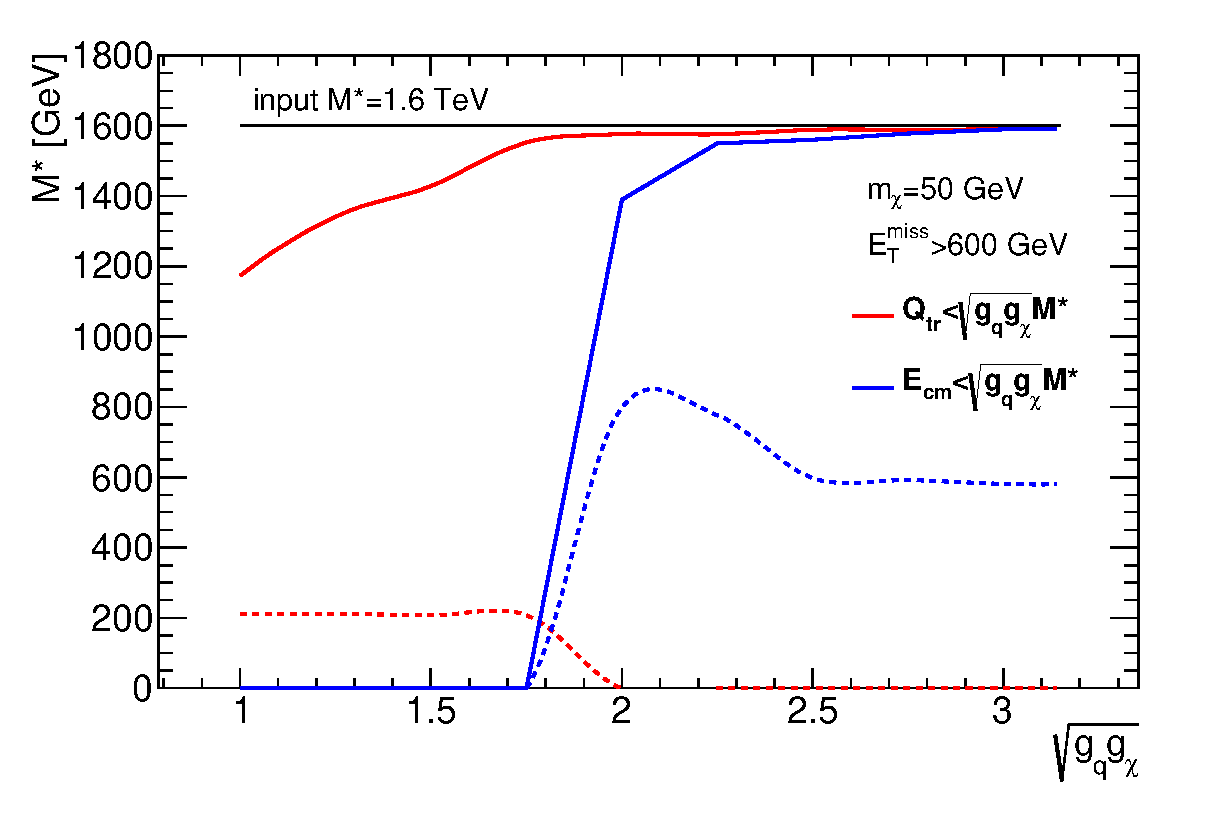
\includegraphics[width=0.95\textwidth]{figures/EFT/MstarvsCouplingSel600_DM_EFT_D5_DM50}
	\caption{95\% CL lower limits on the scale of the interaction of the D5 operator at 14~\tev, after the two truncation procedures. 
		The procedure from~\cite{Racco:2015dxa} outlined in Section~\ref{sec:TruncationWithSHat} is shown in blue, while the procedure from Refs.~\cite{Busoni:2014sya,Aad:2015zva}, described in Section~\ref{sec:TruncationWithQTr} is shown in red. Only the region between the dashed and the solid lines is excluded.}
	\label{fig:monojet_MstarMmed}
\end{figure}

\Todo{This plot needs to be clarified further: what is the statistics for the truncation with sHat, and does this cause the sudden drop at $\sqrt{g}$=2?}

\subsection{Comments on unitarity considerations}
\Todo{Waiting for input from J. Alcaraz}

A further consideration applicable to EFT operators at hadron colliders
is the potential violation of unitarity.  An analysis of the operator
$\displaystyle {\bar{q}\gamma_\mu q\bar\chi\gamma^\mu\chi \over \Mstar^2}$
provides the limit:
\be
\Mstar > \sqrt{s} \sqrt{ {\sqrt{3} \over 4 \pi} \beta(s) },
\ee
where $\sqrt{s}$ is (maximally) the collider energy and $\beta(s)$ is
the DM velocity \cite{Shoemaker:2011vi}.
Constraints for other operators have also been derived \cite{Endo:2014mja}.
This constraint on \Mstar still is open to interpretation, since the
relation to \Mcut is not resolved, except for a specific simplified model.
Derived limits on \Mstar should be compared to this unitarity bound to
check for consistency.


\section{Recommendation for presentation of EFT results} %change this title
\label{sec:RecommendationEFTResults}

In this report,
we make two recommendations for the presentation of collider results
in terms of Effective Field Theories for the upcoming Run-2 searches. 
A full discussion of the presentation of
collider results in relation to other experiments
is left to work beyond this Forum, where ATLAS, CMS, the theory community
and the Direct and Indirect Detection communities are to be involved. 

We divide the EFT operators in two categories: 
those that can be mapped to one or more UV-complete simplified models, such as those
commonly used in LHC searches so far and detailed in~\cite{Goodman:2010ku}, and those
for which no UV completion is available, such as those outlined in Section~\ref{sec:EFT_models_with_direct_DM_boson_couplings}.
%% The For the first case, the EFT is supposed to cover the cases where the mediating particles are heavy,
%% thus overlapping with the simplified models outlined in this report.
%% Results for this first class of operators can be recast starting from simplified models with high mediator masses, 
%% therefore removing the need to explicitly simulate EFT events but still effectively providing experimental limits
%% for those operators. For the second class of models, a truncation procedure 
%% should be applied for various hypotheses on the goodness of the EFT approximation, 
%% and the truncated results presented alongside the full EFT results.

\subsection{EFT benchmarks with corresponding simplified models}
\label{sub:EFT_withSimp}
%% \begin{figure}
%% \centering
%% 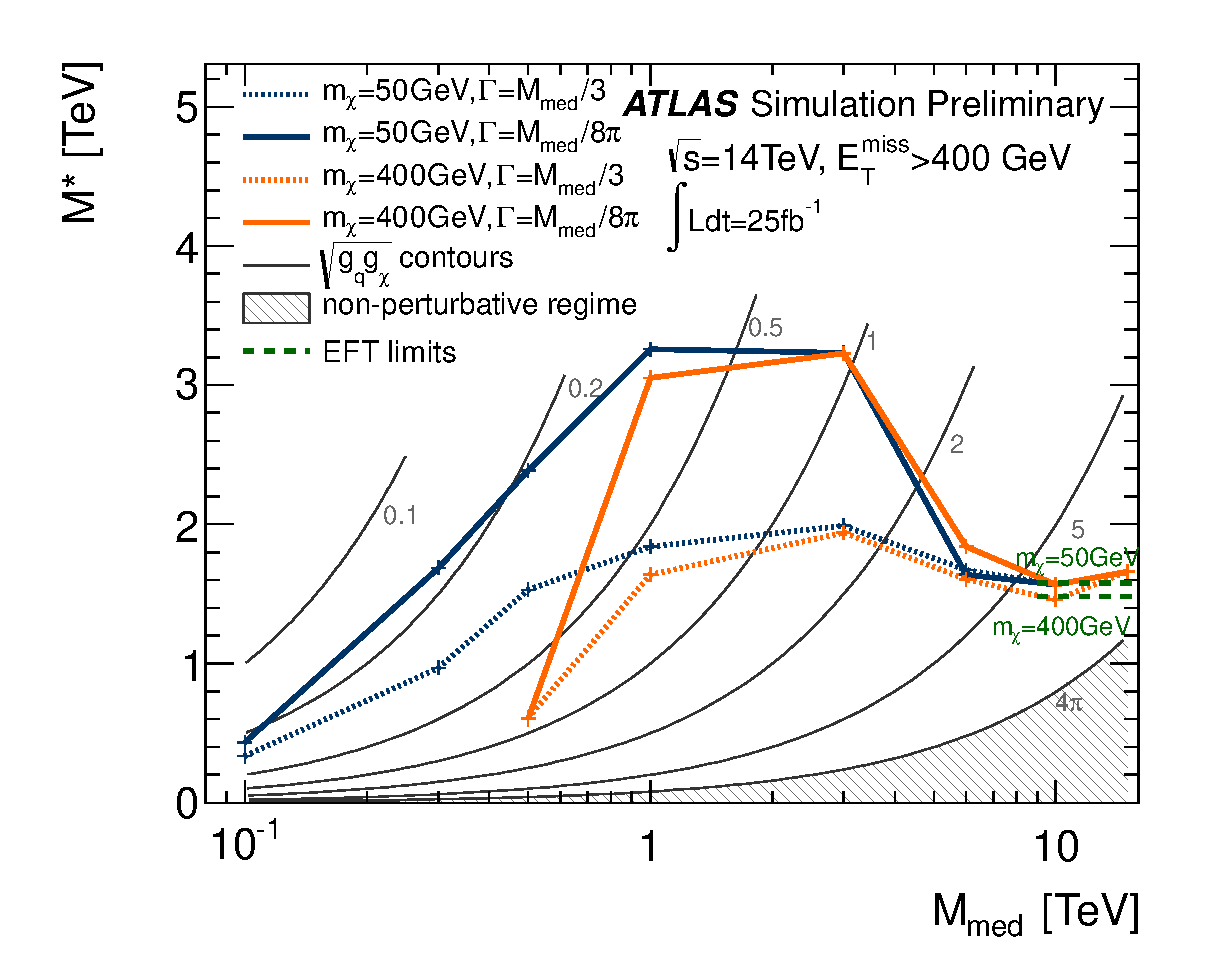
\includegraphics[width=0.9\textwidth]{figures/monojet/lambda_14TeV_SR1.eps}
%% \caption{Comparison of the 95\% CL lower limits on the scale of the interaction of a \Zprime-like simplified model at 14~\tev, in terms of the mediator mass. Corresponding limits from EFT models are shown on the same plot as green dashed lines to show equivalence between the two models for high mediator masses.
%% Taken from Ref.\,\cite{ATL-PHYS-PUB-2014-007}.}
%% \label{fig:monojet_MstarMmed}
%% \end{figure}

If a simplified model can be mapped to a given EFT, then the model's high-mediator-mass limit  will converge to the EFT.
%% This can be seen in Fig.~\ref{fig:monojet_MstarMmed}, where the limits on 
%% the scale of the interaction for a vector mediator exchanged in the \schannel are presented in terms of the mediator 
%% mass~\footnote{This plot only serves to exemplify the convergence of the simplified model to a contact
%% 	interaction operator: before this report, ATLAS and CMS searches presented search results up to very high couplings
%% 	and therefore large widths, potentially probing unphysical corners of phase space}. 
%% It can be seen that the limits at high mediator mass for this model are equivalent to those of the corresponding EFT benchmark.
Numerically, for 14 TeV studies, we have
determined that to fully reproduce the kinematics of a contact
interaction and have no remaining dependence on the presence of a resonance
that is as narrow as the choice made in Section~\ref{sub:parameter_scan_monojet} (\gq = 0.25 and \gDM = 1),
the mediator mass needs to be at least 10 TeV.
A comparison of the main kinematic variables for the \schannel vector 
mediator model with a width of 0.1 \mMed
is shown in Fig.~\ref{fig:EFT_kinematics}.\footnote{The use of a fixed width rather than the minimal width is exclusive of these plots.} 

%CD: do we want to add more of the discussion here on why this happens? I would personally keep it short.

\begin{figure}[hbpt!]
	\centering
	\subfloat[\MET{}]{
		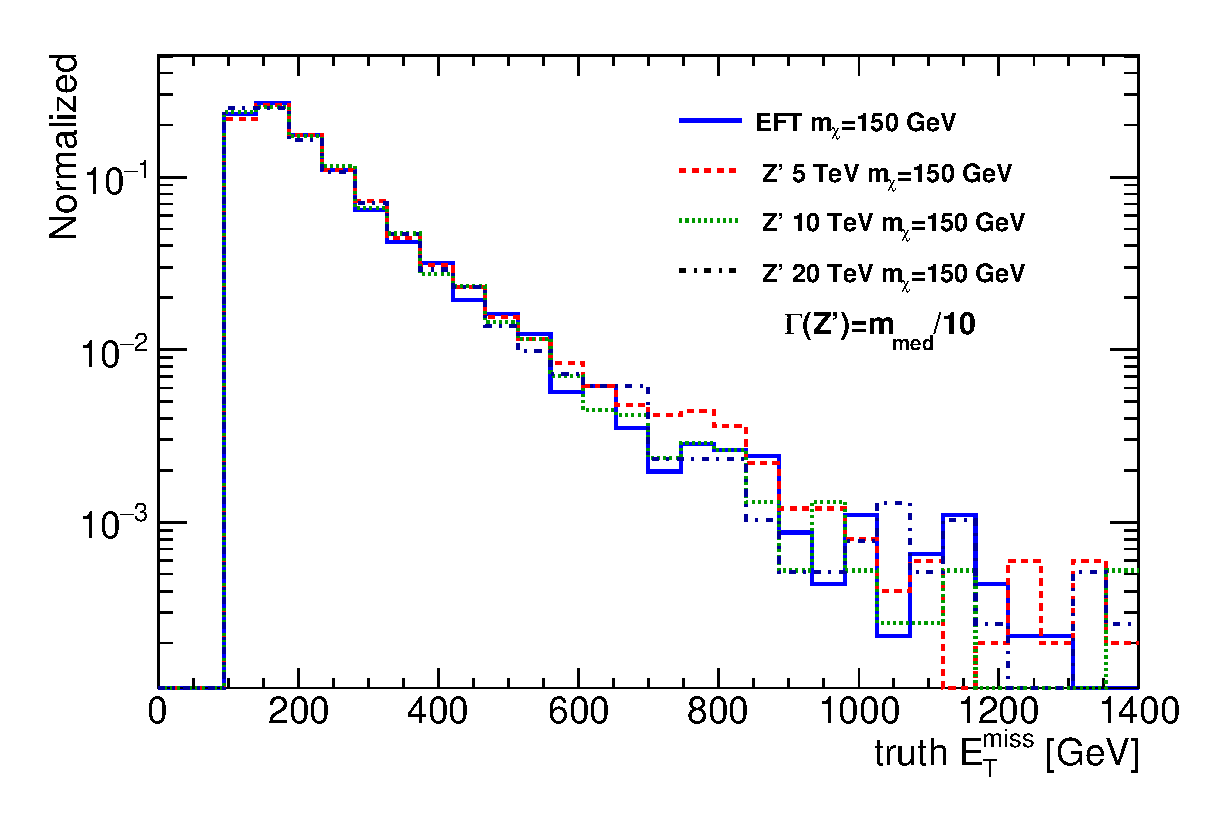
\includegraphics[width=0.7\linewidth]{figures/EFT/TruthETmiss_compEFTvsZprime_DM150_narrow.eps}
	}
	\caption{Comparison of the kinematic distributions at 14~\tev between a narrow \schannel mediator and the
	corresponding D5 contact operator, at generator level for a jet+\MET{} signature. 
	\label{fig:EFT_kinematics}}
\end{figure}
%\vskip-50pt %UGLLYYYYYYY
\begin{figure*}[ht!]
	\setcounter{subfigure}{1}
	\centering
%	\subfloat[\MET{}]{
%		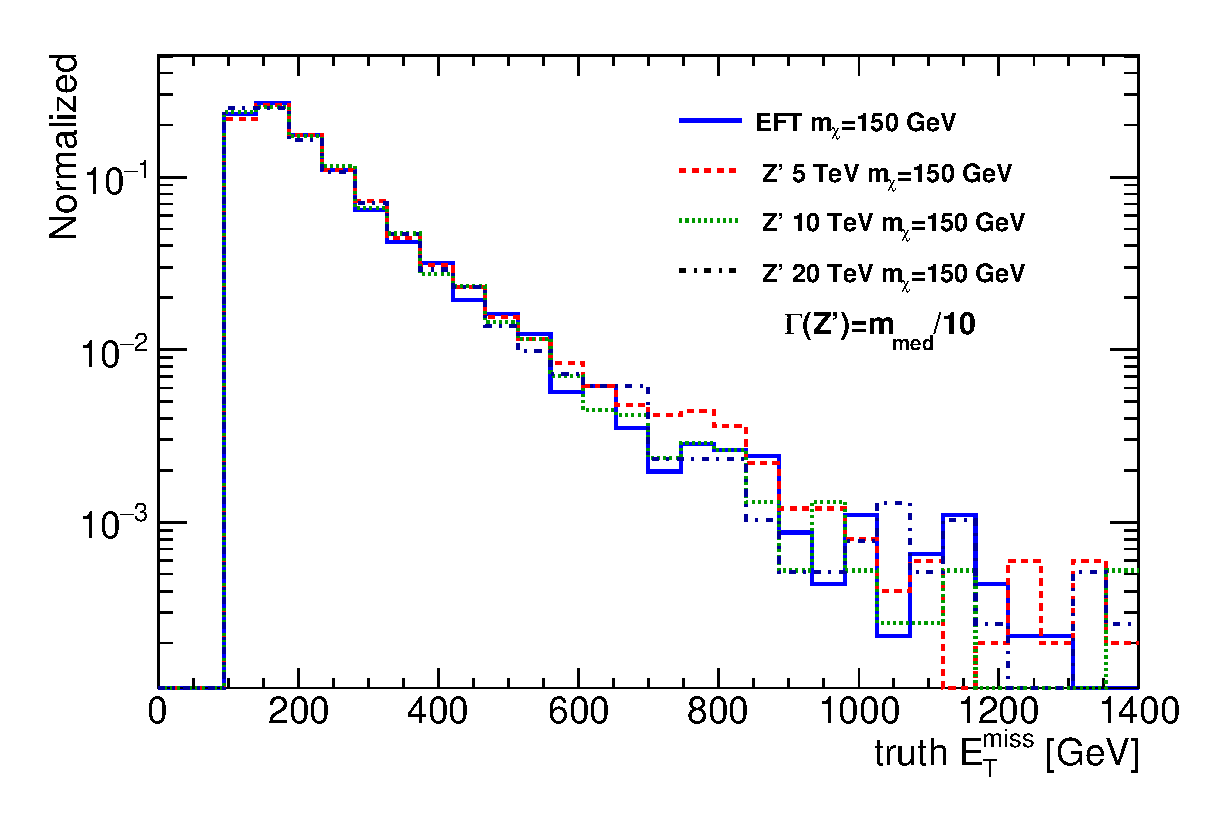
\includegraphics[width=0.7\linewidth]{figures/EFT/TruthETmiss_compEFTvsZprime_DM150_narrow.eps}
%	}
	\subfloat[Center of mass energy $E_{cm}$]{
	   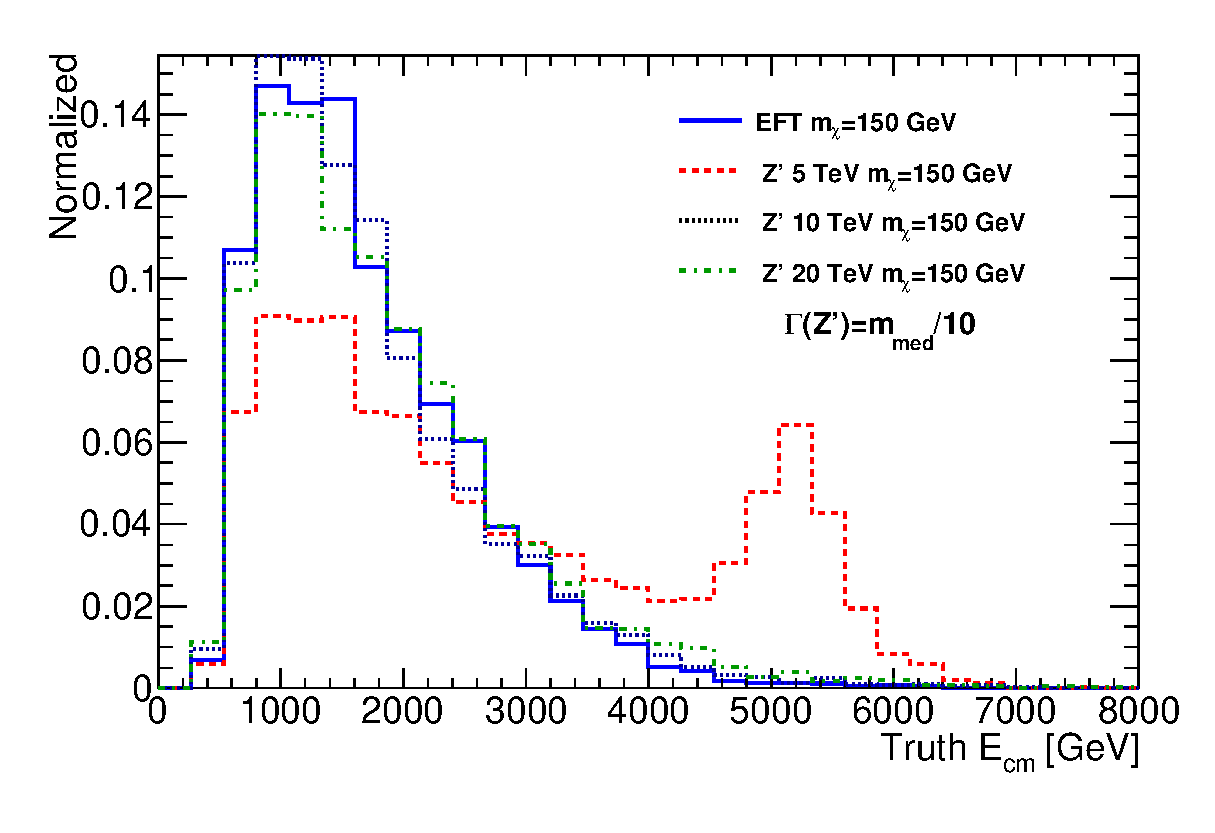
\includegraphics[width=0.47\linewidth]{figures/EFT/TruthEcm_compEFTvsZprime_DM150_narrow.eps} 
	}		
	\subfloat[Mediator transverse momentum]{
		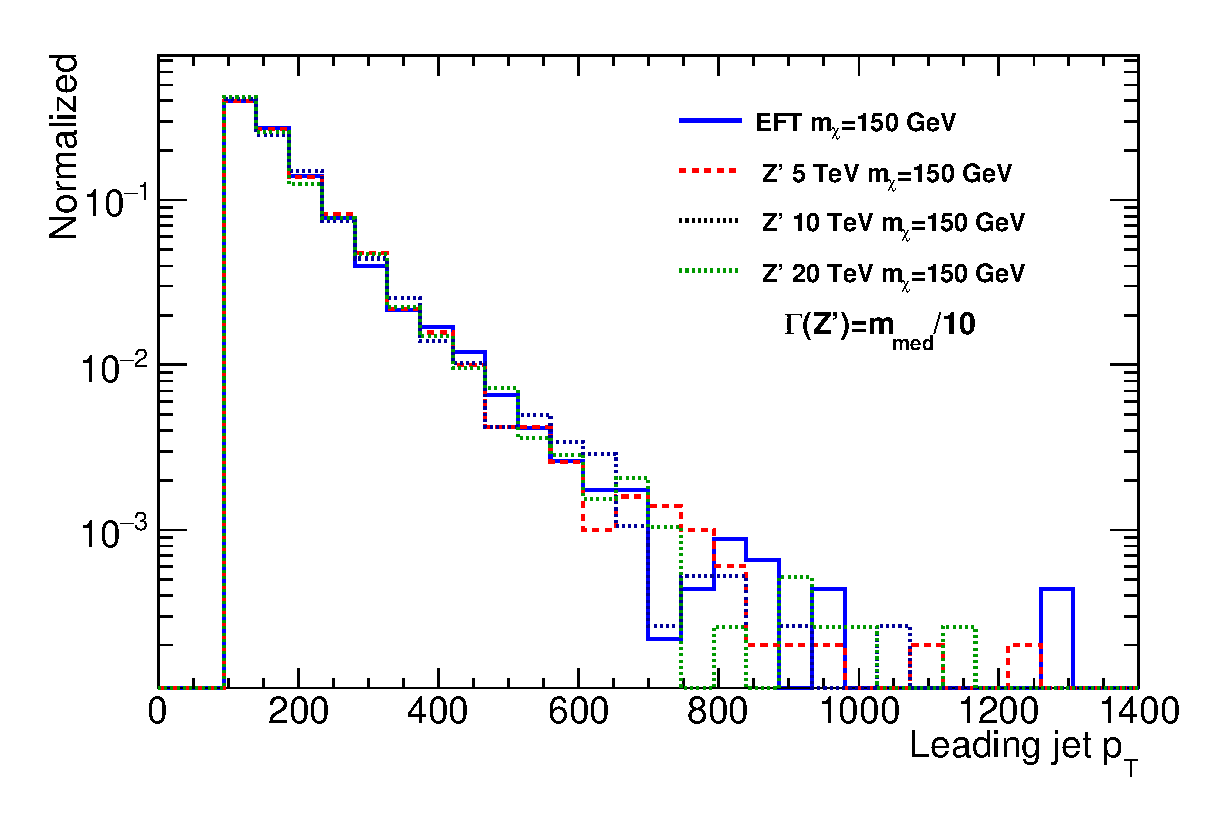
\includegraphics[width=0.47\linewidth]{figures/EFT/TruthPt_compEFTvsZprime_DM150_narrow.eps}
	}
		\hfill
	\subfloat[DM transverse momentum (leading)]{
		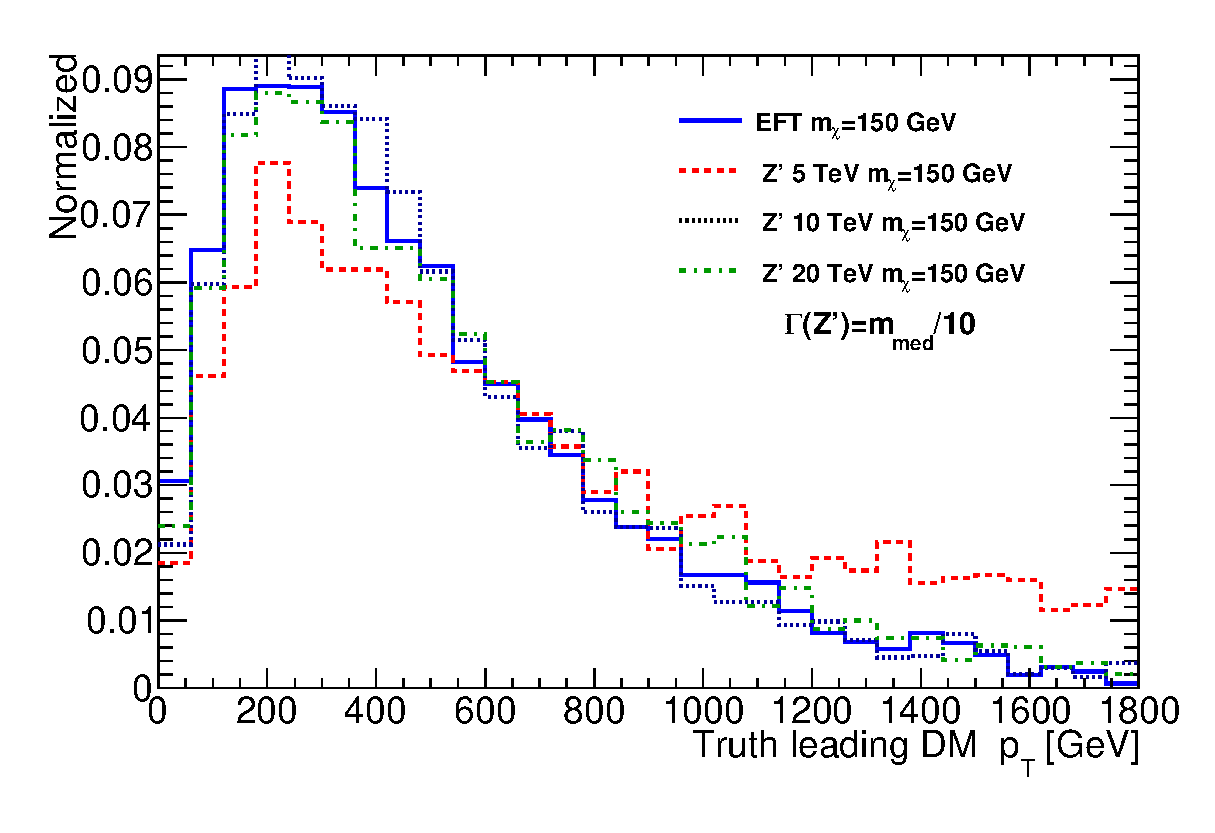
\includegraphics[width=0.47\linewidth]{figures/EFT/TruthDM1ptcompEFTvsZprime_DM150_narrow.eps} 
		}
	\subfloat[DM transverse momentum (sub-leading)]{
		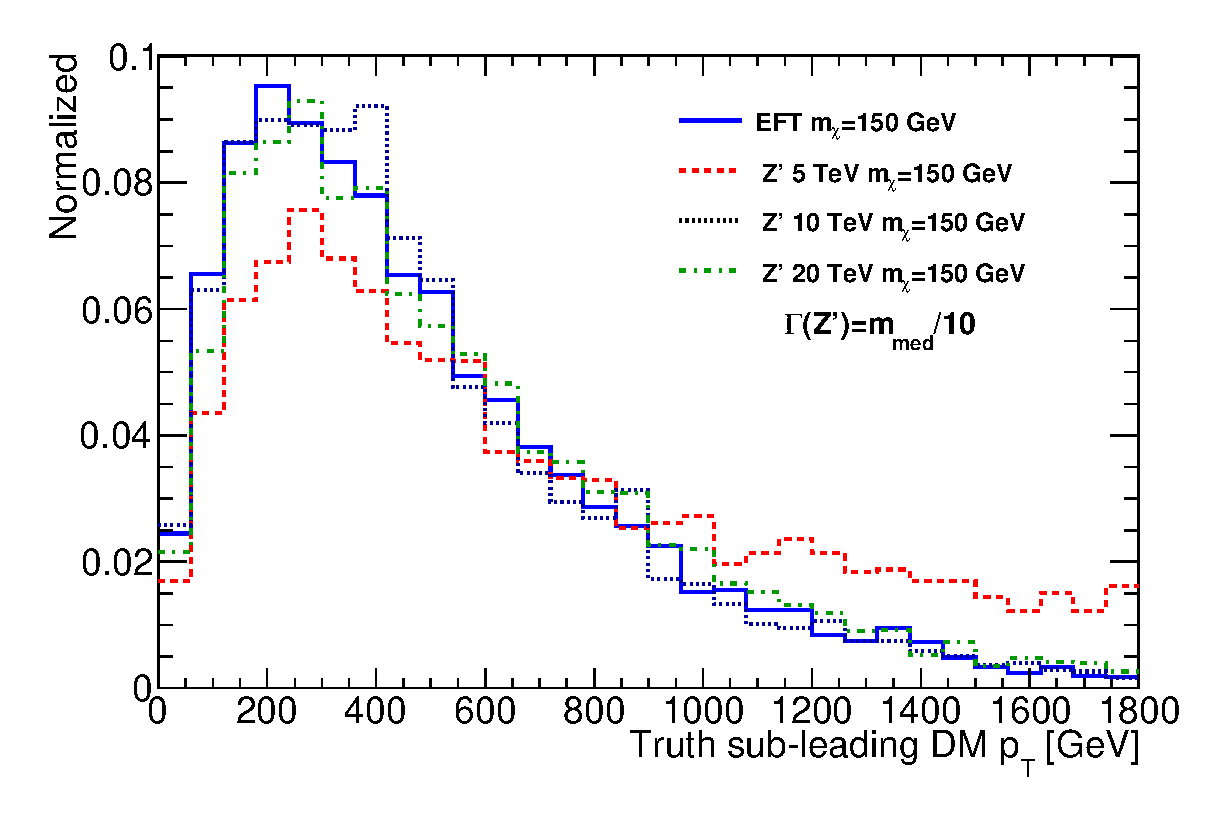
\includegraphics[width=0.47\linewidth]{figures/EFT/TruthDM2ptcompEFTvsZprime_DM150_narrow.eps} 
	}
\end{figure*}


%\Todo{We may get plots with a width.mass ratio of 0.05, which is closer to the minimal width.}

As already observed in Section~\ref{sub:parameter_scan_monojet}, varying the DM mass changes the kinematics,
both in the simplified model and in the EFT case. This can be seen in Fig.~\ref{fig:EFT_kinematics_mDM}. 

\begin{figure*}[hbpt!]
	\centering
	\subfloat[\MET{}, D5 operator]{
		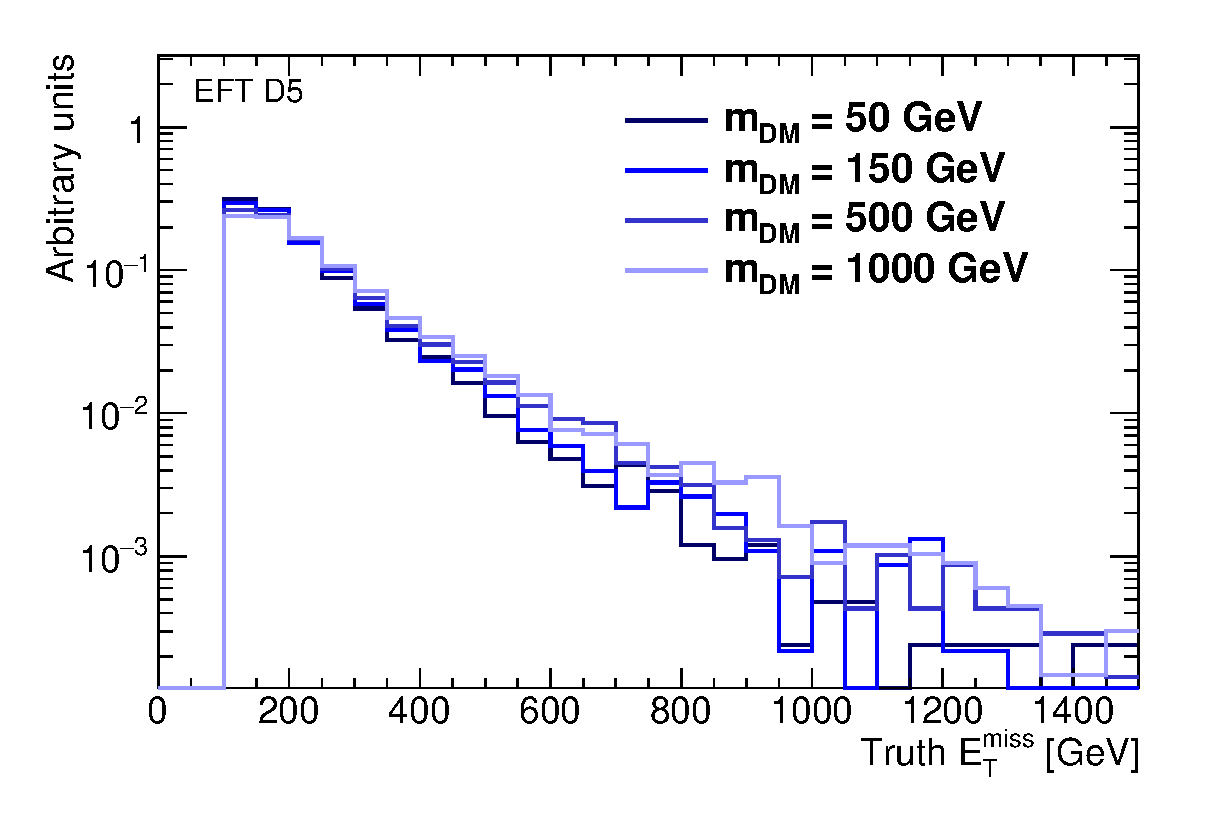
\includegraphics[width=0.47\linewidth]{figures/EFT/EFT_met}
	}
	\subfloat[Invariant mass of the two WIMPs $m_{\chi \chi}$, D5 operator]{
		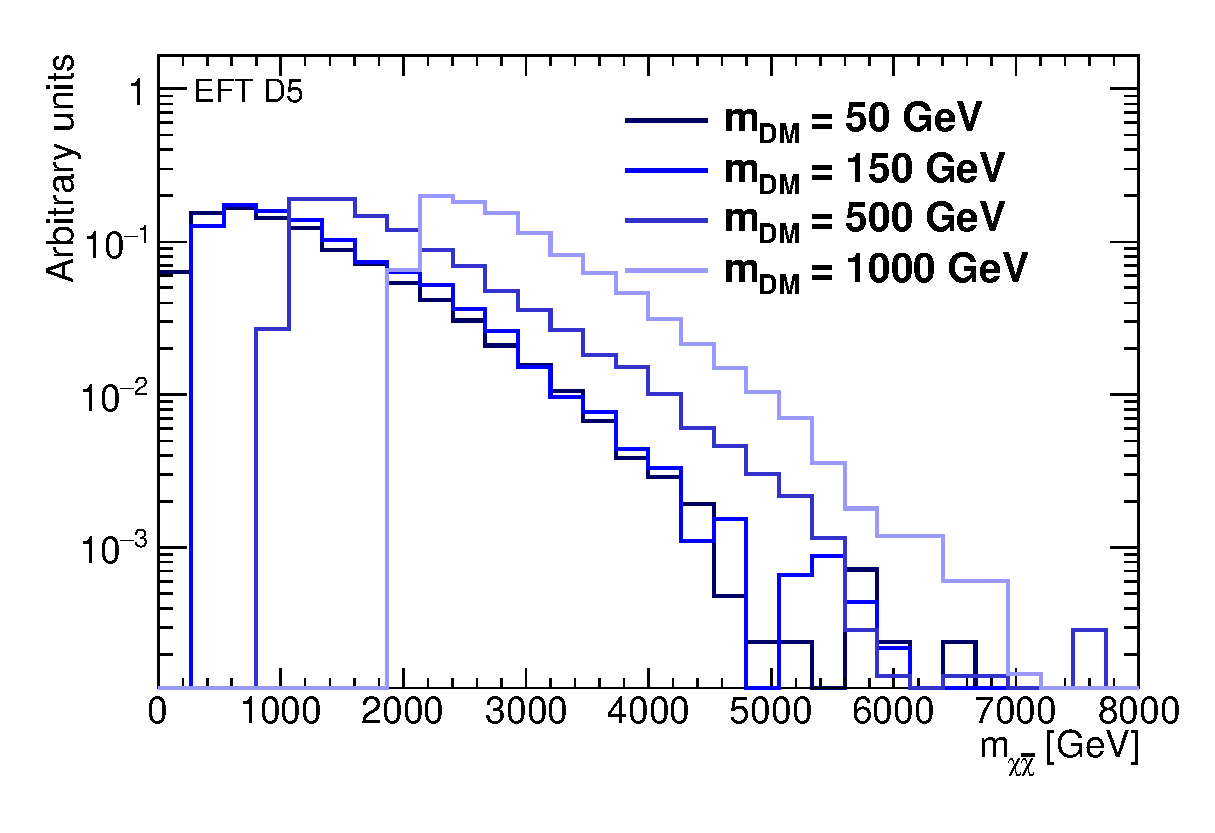
\includegraphics[width=0.47\linewidth]{figures/EFT/EFT_shat} 
	}		
	\hfill
	\subfloat[\MET{}, simplified model]{
		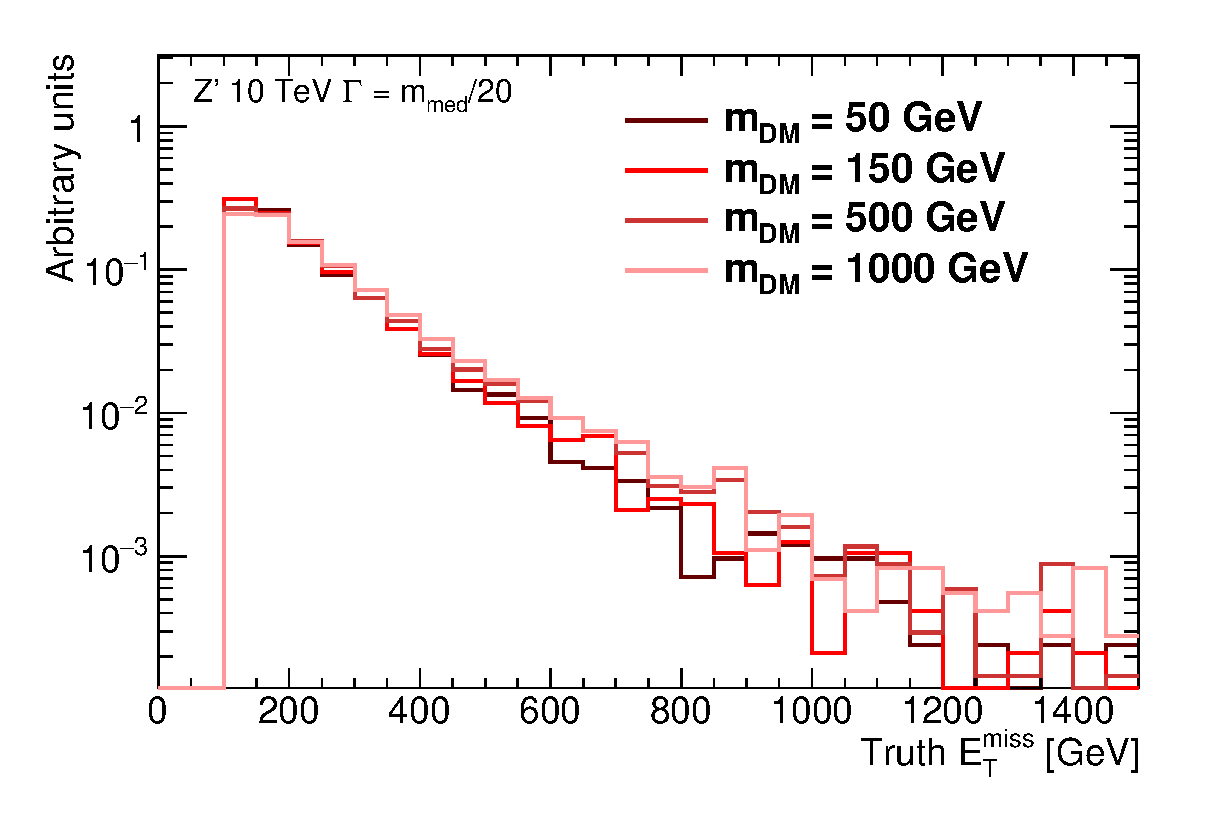
\includegraphics[width=0.47\linewidth]{figures/EFT/Zprime_met}
	}
	\subfloat[Invariant mass of the two WIMPs $m_{\chi \chi}$, simplified model]{
		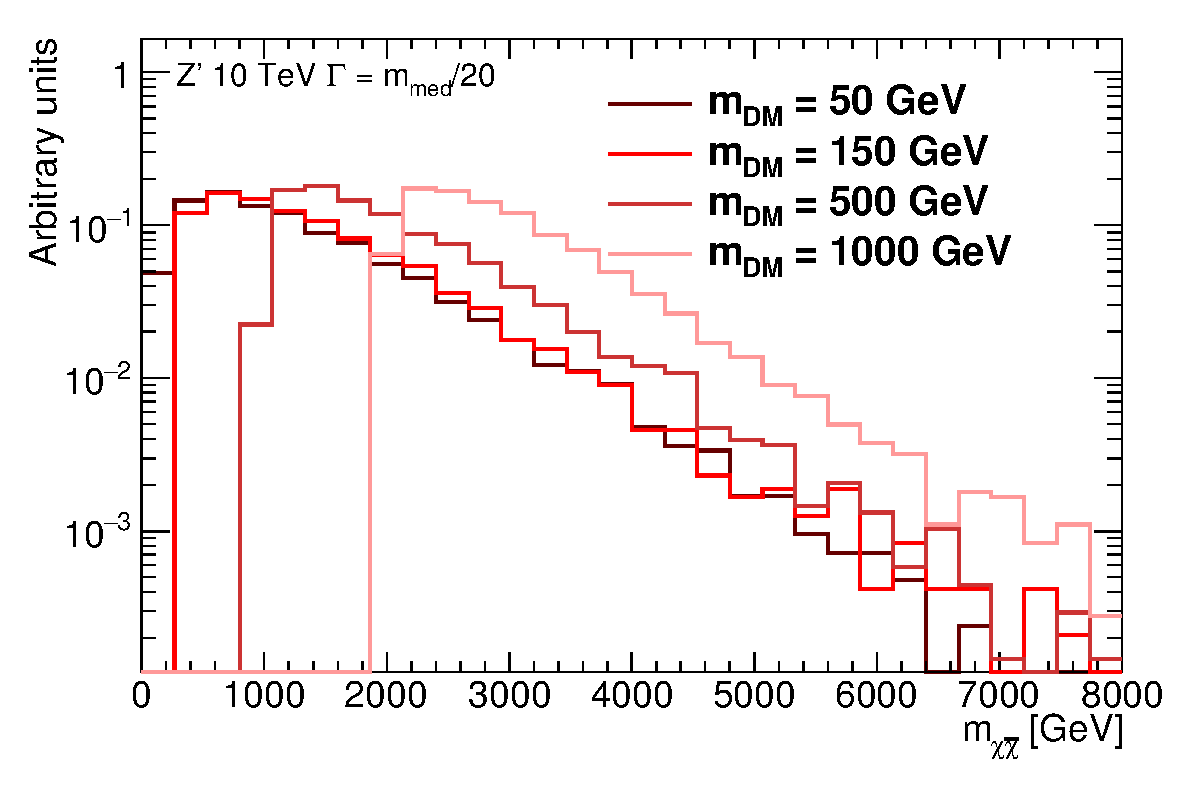
\includegraphics[width=0.47\linewidth]{figures/EFT/Zprime_shat} 
	}		
	\caption[][28pt]{Comparison of the kinematic distributions for a narrow \schannel mediator, 
		at generator level for a jet+\MET{} signature, for varying DM masses. 
		\label{fig:EFT_kinematics_mDM}}
\end{figure*}

\vskip20pt
	
Based on these studies, the Forum recommends experimental collaborations to deliver 
results for mediators with a mass of 10 TeV instead of fully simulated EFT results for each of the DM masses 
considered in the scan, and leave further reinterpretation to theorists.
It should be checked that the high-mass mediator case for the simplified model is correctly implemented 
We therefore advise to add one grid scan point at very high mediator mass (10 \tev) to the scan, 
for each of the DM masses for the simplified models described in Section~\ref{subsec:MonojetLikeModels}. 
%The truncation procedure in Section~\ref{sec:TruncationWithSHat} can be used to fine-tune the mediator mass to be simulated for this purpose. 

%\Todo{The extrapolation to other couplings and mediator masses can be
%	done using the \Qtr prescription for that model. CD: I think this was Steve M - what do you mean?}

\subsection{EFT benchmarks with no corresponding simplified models}

%% Three proposals for the treatment of EFT have been stated so far,
%% to complement raw EFT results: (1) truncate using \Qtr, (2) truncate and iterate using \Qtr, and
%% (3) truncate using \Ecm.  The reliability of the EFT approximation can
%% also be quantified by presenting the sensitivity of the results to \Reft, the fraction of events
%% that satisfy $\hat{s} > \Mcut ^2$, for example.

Whenever a UV completion is not available, EFT results are still
a source of useful information as 
described in Section~\ref{sub:validityEWContact}. 
However, we can only roughly control how well the EFT approximation holds.
Despite the fact that a propagator was introduced to motivate
the truncation procedure for \schannel models, the prescription from Sec.~\ref{sub:EFT_withSimp}
depends upon the simplified model to derive the
energy scaling that is used for the comparison with the momentum transfer. 
The simple fact remains that the effective
coupling of the operator -- $g/\Lambda^n$ -- should not allow
momentum flow $Q>\Lambda$ or $g>4\pi$.  Given our ignorance of
the actual kinematics, 
the truncation procedure recommended for this purpose
is the one described in Section~\ref{sec:TruncationWithSHat},
as it is independent from any UV completion details. 

Because there is no UV completion,
the parameter \Mcut can be treated more freely than
an explicit function of $g$ and $\Lambda$.
It makes sense to choose \Mcut such that we 
identify the transition region where the EFT stops being
a good description of UV complete 
theories. This can be done using the ratio \Reft, which is defined
as the fraction of events for which $\hat{s} > \Mcut^2$. 
For large values of \Mcut, no events are thrown away in the truncation 
procedure, and \Reft = 1. As \Mcut becomes smaller, eventually all events are thrown 
away in the truncation procedure, i.e. \Reft = 0, and the EFT gives no 
exclusion limits for the chosen acceptance.  

We propose a rough scan over \Mcut, such that we find the values of \Mcut 
for which \Reft ranges from 0.1 to 1. The analysis can then perform a scan over 
several values of \Mcut, and show the truncated limit 
for each one of them alongside the naive limit corresponding to \Reft = 1. 

%When \Reft=0, there is no limit. When \Reft reaches 1, the truncated limit 
%is identical to the original limit. (<== These last two sentences may be overkill. 
%Cut it if you think this is already clear)

